\subsection{Run on The Cancer Genomics Atlas}
The same pipeline described so far can be applied at other datasets. In this section, the hSBM model is run on some samples from the TCGA. The principle is the same, but here samples come from cancer tissues, so there must be more complexity and variability behind the data. Moreover, being able to separate cancer samples is not always easy clinically and develop a method to do this can be highly interesting and useful for the scientific community~\cite{Farver2018}. 

First of all, let's take a look at the V-measure scores. As shown in figure~\ref{fig:topic/tcga/metric} the score is almost $0.7$, which is good, but worse than the healthy GTEx scenario. In this dataset, there isn't a sub-tissue label as before, but a disease type cancer information is available. The disease type separation is not so good; the fact that there is no evident difference between Zipf's laws when separating data by disease type~\ref{fig:structure/tcga/fraction_of_trascriptome_disease} means that all genes contributes to define this specific label so the pre-process filter is not a good option in this case. To gain better scores in this situation where samples are affected by the cancer complexity and heterogeneity is probably necessary to add more genes to the network.
\begin{figure}[htb!]
    \centering
    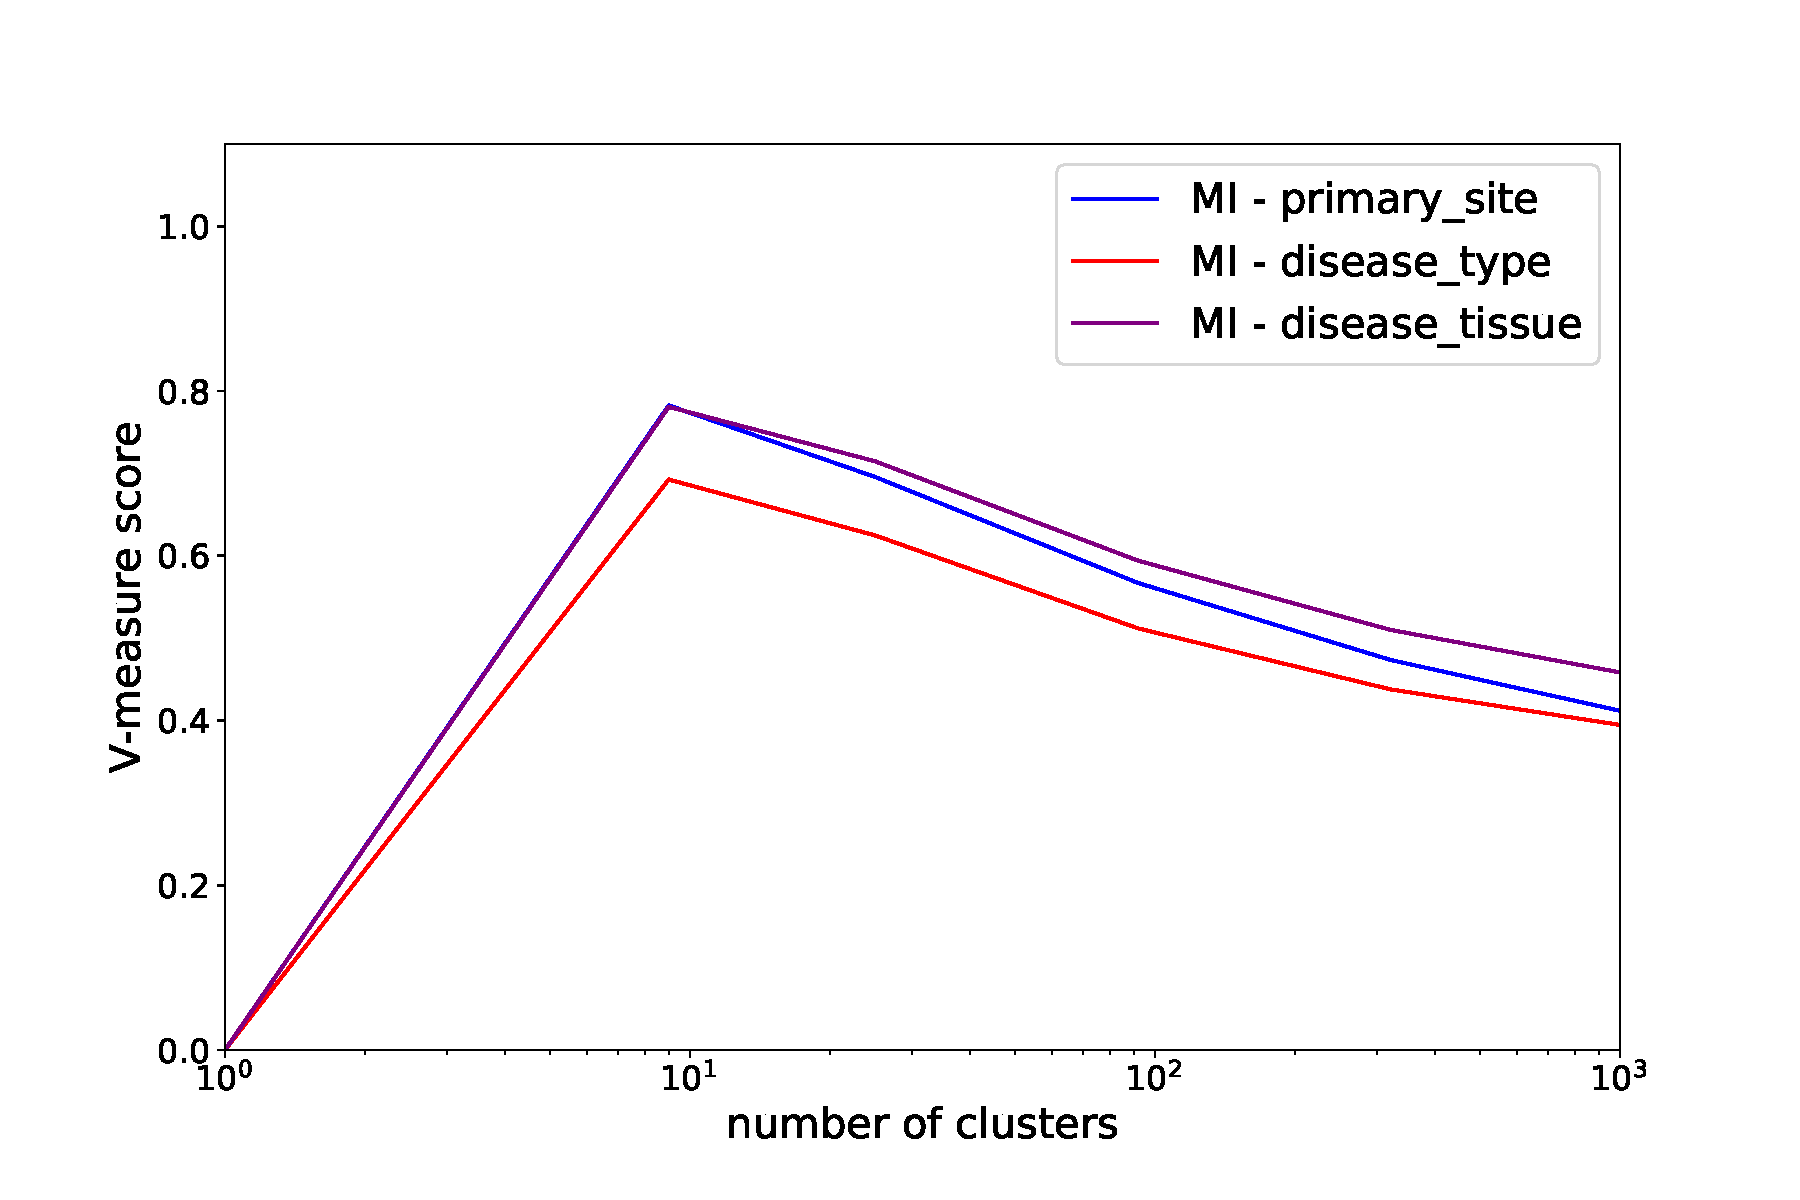
\includegraphics[width=0.8\linewidth]{pictures/topic/tcga/metric.pdf}
    \caption{Score across the hierarchy for TCGA. In blue the primary site labels were considered, in red the disease types and in purple the mix of the two.}
    \label{fig:topic/tcga/metric}
\end{figure}

Looking directly into the cluster composition the tissue separation is quite good and visually appreciable. In figure~\ref{fig:topic/tcga/fraction_clustercomposition_l4_primary_site} clusters at the higher level of the hierarchy. Some tissues are well separated at this point, at the same time when possible samples are grouped by system, digestive system is the more evident.
\begin{figure}[htb!]
	\centering
	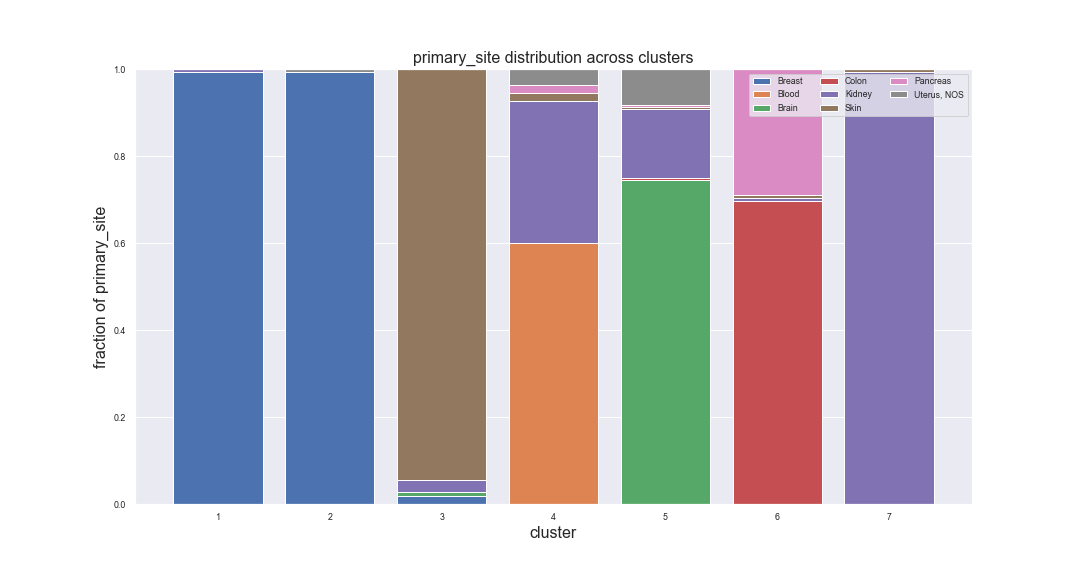
\includegraphics[width=0.8\linewidth]{pictures/topic/tcga/fraction_clustercomposition_l4_primary_site.png}
	\caption{Clusters of diseased tissues at the higher level of the hierarchy. Breast is well separated, such as skin and brain. Cluster 6 contains digestive systems samples from pancreas and colon.}
	\label{fig:topic/tcga/fraction_clustercomposition_l4_primary_site}
\end{figure}
Going deeper in the hierarchy the tissue separation becomes visually appreciable and all the clusters are almost tissue-specific.
\begin{figure}[htb!]
	\centering
	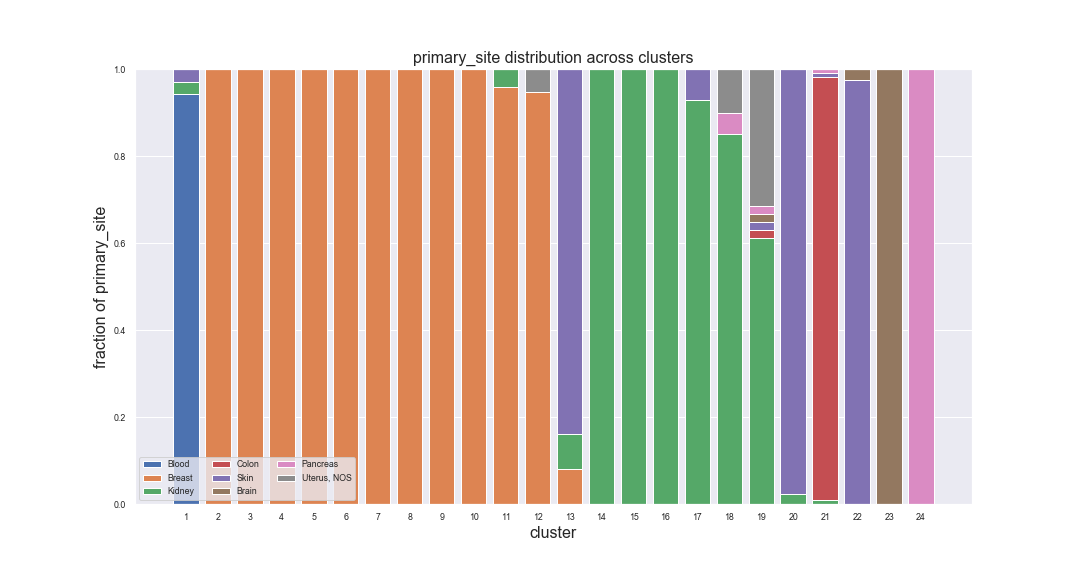
\includegraphics[width=0.8\linewidth]{pictures/topic/tcga/fraction_clustercomposition_l3_primary_site.png}
	\caption{Normalized cluster composition from diseased samples.}
	\label{fig:topic/tcga/fraction_clustercomposition_l3_primary_site}
\end{figure}
\FloatBarrier
At this point when the model is demonstrated to work on healthy and diseased samples, it can be interesting to study merged healthy and diseased labels and examine how the model behaves when healthy and cancer samples are merged.